\chapter{Introduction}

Electronic mail or email is one of the most common digital communication tool used currently. A survey conducted on Internet users in the US in 2010 indicated that 94\% of them have used email as a communication tool. It also suggested that 62\% of them use emails daily. These numbers have significantly grown since 2010~\cite{1} . Rise in the amount of emails exchanged has attracted significant number of spammers. Email spam is unsolicited bulk email. Spam e-mails pose as a serious threat to the usefulness and popularity of email which contains advertisements, malware, phishing links, adult content, etc. 

\par In the nascent stages, email spam was seen in the form of text emails. Several successful classifiers were developed to filter spam emails based on content, subject, header, etc. Lai and Tsai~\cite{2} explore 4 Machine Learning algorithms used to build classifiers using different parts of the email like content, body, header, etc. Machine Learning algorithms like Naive Bayes, Support Vector Machines (SVM), k-Nearest Neighbors (KNN), etc. have been widely used in email spam detection.

\par With stronger text based classifiers being developed to filter spam emails, spammers invented various other techniques like blank spam, image spam and backscatter spam to evade text based detection. Email spam sent in the form of images is commonly known as email image spam or image based spam. Spam text is embedded inside images making it easier to evade text based detection~\cite{3}. ``Spam now accounts for 90.4 percent of all e-mail, according to a report released Monday from security vendor Symantec''~\cite{4}. 

\par Initial image spam was seen in the form of simple text converted to images. Optical Character Recognition (OCR) can be used to extract text inside an image. This text is then subjected to text based detection techniques. To evade OCR based detection scheme, spammers introduced obfuscation techniques in spam images which prevent OCR from reading the text embedded inside the images~\cite{5}. 

\par This opened a whole new avenue for research in image spam detection techniques. Image processing techniques were introduced for image spam detection. Detection schemes are now developed using multiple image properties as input to machine learning algorithms. 

\par In this research, we will explore how image processing can be used in conjunction with machine learning algorithms. Fig. \ref{fig:architecture}. shows the basic architecture of the proposed research. Since there are very limited public datasets available for image spam research, we developed a synthetic dataset. The aim of constructing this dataset was to challenge the detection scheme we developed. 

\begin{figure}
	\centering
	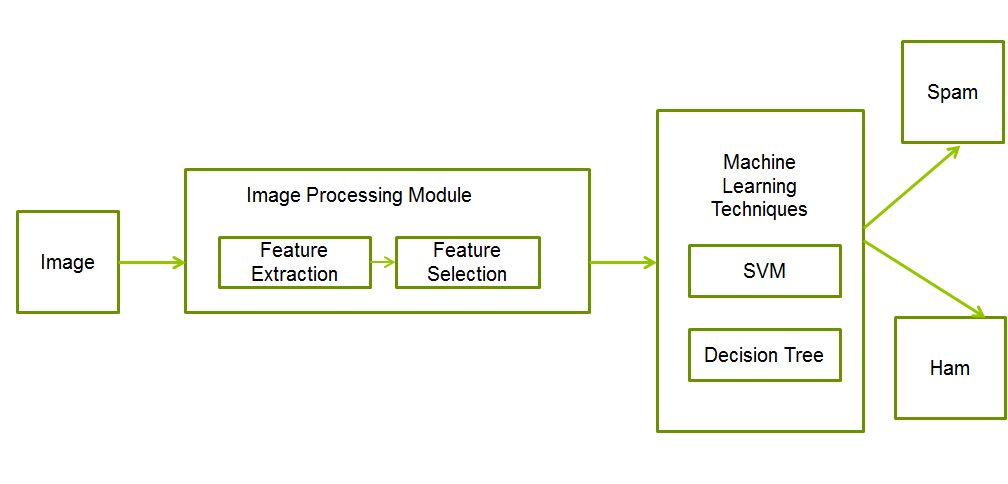
\includegraphics[width=\textwidth]{images/architecture}
	\caption{Proposed Architecture}
	\label{fig:architecture}
\end{figure}

\par In chapter 2 we give a brief overview about what is image spam, detection techniques and related work done in this domain. In chapter 3, we talk about image features used in the experiments. Chapters 4 and 5 give a brief overview about datasets and machine learning model used for the experiments. Chapter 6 details the environmental setup. In chapter 7, we discuss the process of generating the synthetic dataset and evaluate it. Chapter 8 dives into the experimental results of SVM Model with the datasets.
